\section{Server Secuirty}

Man sollte davon ausgehen, dass die verwendete Software Schwachstellen besitzt. Auch wenn diese Schwachstellen nicht ausreichen, können sie dennoch als Sprungbrett für andere Angriffe verwendet werden. Daher ist es zwingend Nötig, das System auf allen möglichen Ebenen zu Härten und damit die Sicherheit zu erhöhen. Man spricht dabei von einer \textbf{Multi-Defense Strategy}.\\

Statistisch gesehen existiert für eine neu entdeckte Sicherheitslücke nach \textbf{6 Tagen ein Exploit} und erst \textbf{nach 54 Tagen ein Patch}. Oftmals ist Lesezugriff ausreichend, um einem Unternehmen Schaden zuzufügen oder daraus zu profitieren. Schreibzugriffe sind ebenfalls nicht zu vernachlässigen.\\

Besitzt der Angreifer Schreibzugriff, so kann er Anwendungen auf den Server laden und diese später ausführen. Beispiel: PHP Shell.

\subsection{XXE File Inclusion}
Unter dem Begriff ist eine Attacke über das \textit{XML External Entity Processing} möglich. Dabei können externe Daten, wie z.B. lokale Dateien, in das XML inkludiert werden. Bei der Verarbeitung solcher Inclusions, welche im DTD angegeben sind, fügt sie der Parser in die angegebenen Stelle ein.\\

\textbf{Lösung:} Deaktivierung des Features für DTDs (External Entities) beim Parser.

\begin{lstlisting}[language=XML, caption=Beispiel der XXE]
<?xml version="1.0" encoding="ISO-8859-1"?>
<!DOCTYPE foo [  
  <!ELEMENT foo ANY >
  <!ENTITY xxe SYSTEM "file:///etc/passwd" >]><foo>&xxe;</foo>
\end{lstlisting}

\todo[inline]{XXE in eigenes Kapitel verschieben, zusammen mit JSON-Highjacking und URL-Redir.}

\subsection{Hardening}

\subsubsection{Während der Installation des Systems}
\begin{easylist}[itemize]
	& Minimales System
	& Keine Standard-Pfade
	& Separate Disk/Partition für log files
	& Aktuellste Patches eingespielt
	& Default Secure (Umask, Path)
	& Verwendung eines Install Servers
\end{easylist}

\subsubsection{Netzwerksicherheit}
\begin{easylist}[itemize]
	& Nur benötigte Dienste starten
	& Least File Permissions für Dienste anwenden
	& Least Process Privileges anwenden
	& Standard-/Beispielinstallationen entfernen
	& Banner Hiding (keine Versionsinformationen sichtbar)
	& Error Handling (keine Fehlerdetails sichtbar nach aussen)
\end{easylist}
\subsubsection{Authentifizierung}
\begin{easylist}[itemize]
	& Verwendung einer sicheren Authentifizierung (Benutzername, Kennwort, OTP, Client Certificate)
	& Password Policy (Stärke, Gültigkeitsdauer, Kennwortwechsel, Erkennung von Attacken auf geknackte Passwörter)
\end{easylist}
\subsubsection{Monitoring und Auditing}
\begin{easylist}[itemize]
	& Zeitsynchronisation
	& Integritätstests
	& Event handling (info, debug, error, panic, log)
	& Forensic Readiness
	& Remote Logging
\end{easylist}

\subsection{Unix Process Security}
Unter Linux ist ein weit verbreiteter Ansatz in der Prozess-Sicherheit die \textbf{Isolierung durch Chroot} (change root). Dabei wird dem Prozess ein angegebenes Verzeichnis als Root vorgegaukelt. Innerhalb des neuen Root-Verzeichnis befinden sich alle für den Service nötigen Dateien. Er kann dabei nicht auf Dateien zugreifen, welche sich ausserhalb des neuen Root-Directories besitzen. Man spricht dabei auch von einem Jail.

\subsection{File Permissions}
Die Berechtigungen auf Dateisystemebene sollten so restriktiv wie möglich sein. Als Grundsatz gilt: \textbf{Never give "'world"' write access}. Dasselbe gilt für sensitive Informationen: \textbf{Keep sensitive data secure by removing read access from "'world"'}.\\

Um die Standard-Berechtigungen unter Unix zu setzen, kann mit einer Maske gearbeitet werden. Diese ist auch bekannt als "'Umask"'. Um die obigen Berechtigungen für den aktuellen Prozess zu ändern, kann z.B. \lstinline|$ umask 027|.

\begin{figure}[H]
	\centering
	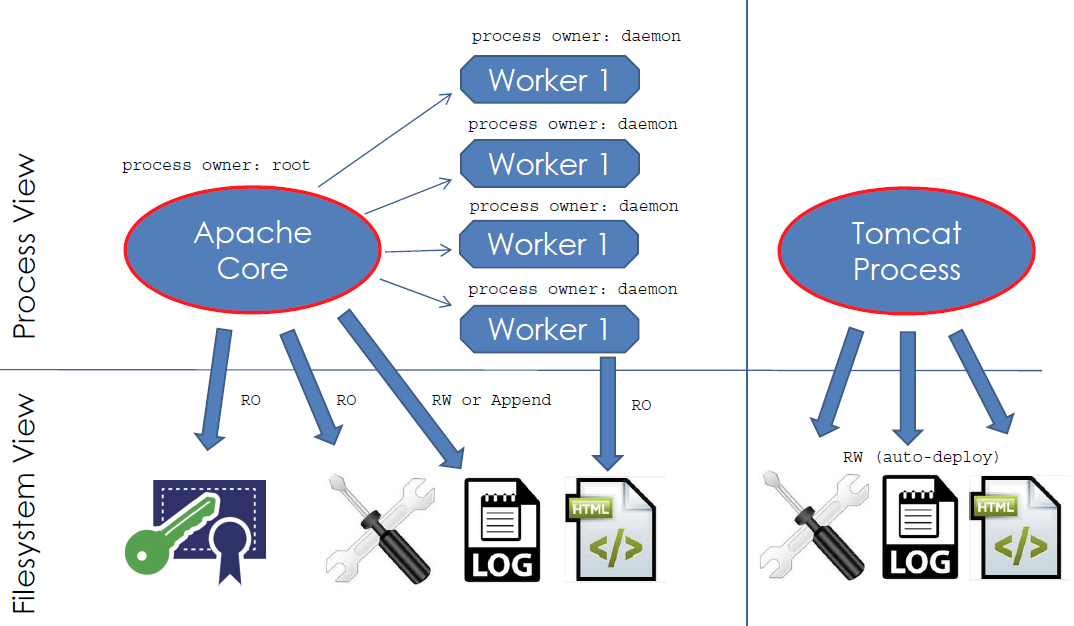
\includegraphics[width=\textwidth]{./img/apache_tomcat_permissions}
	\caption{Beispiel der Berechtigungen für Apache und Tomcat}
\end{figure}

\subsubsection{Apache File Permissions}
\begin{easylist}[itemize]
	& Im Besitz von Root
	&& Konfigurationsdateien
	&& SSL Schlüssel
	&& Log
	&& Html
	& Eigentümer des Apache Prozess benötigt nur RO
	&& Html
\end{easylist}

\subsubsection{Tomcat File Permissions}
Dies gestaltet sich oftmals schwierig, denn Tomcat besitzt eine andere Prozess-Architektur. Der Eigentümer des Tomcat-Prozess benötigt RW, für Remote Deployment, Konfiguration und Load Balancing.

\subsection{Privilege Escalation}
Dabei versteht man die Möglichkeit, die Berechtigungen des aktuellen Prozesses so zu verändern, dass man Zugriff auf andere geschützte Elemente erhält. Dazu können z.B. Bugs in SetUID-Tools verwendet werden.\\

Aber auch CRON kann gefährlich sein, da die Prozesse als Root gestartet werden. Wenn nun ein von CRON-Skript "'world-writeable"' ist, kann somit schnell etwas mit höchsten Berechtigungen ausgeführt werden.

\subsection{Network Hardening}
\textbf{Nur die nötigsten Dienste} sollten gegen Anfragen von aussen reagieren. Alle anderen müssen an \textit{localhost} gebunden sein. Alternativ kann auch eine \textbf{Firewall} dafür eingesetzt werden.\\
Dienste wie UPNP, Bonjour / Zeroconf und DLNA sollten aufgrund ihrer grossen Attach-Surface auch deaktiviert werden. Dies stammt daher, dass oftmals die Geräte unzureichende Authentifizierungsmechanismen implementiert haben.\\

Es wird in den Folien auch von der \textbf{Verwendung von IPv6 abgeraten}.\\

\textbf{ICMP-Redirects deaktivieren}, um MITM-Attacken vorzubeugen.\\

Eine Analyse mittels Nmap oder \href{https://cisofy.com/lynis/}{Lynis von Cisofy} helfen, Schwachstellen aufzudecken.

\todo[inline]{AIDE}
\todo[inline]{DB Hardening}